\documentclass{article}
\usepackage[T1]{fontenc}
\usepackage{lmodern}
\usepackage{graphicx}
\usepackage{amsmath,amssymb}
\usepackage[a4paper,margin=2cm]{geometry}
\usepackage[absolute,overlay]{textpos}
\setlength{\TPHorizModule}{1mm}
\setlength{\TPVertModule}{1mm}
\usepackage[indonesian]{babel}
\usepackage{hyperref}
\setlength{\emergencystretch}{2em}
% unit: Halaman 59

\begin{document}

% === Halaman 59 (python/native) ===

• Sedangkan di dalam cipher blok yang lain, permutasi tidak menggunakan P-box, 

tetapi melakukan pergeseran bit ke kiri atau ke kanan sejauh k bit.

• Pergeseraran bersifat siklik, yaitu bit yang paling ujung muncul pada ujung yag 

lain

• Contoh pergeseran byte di dalam AES:

59

% deskripsi: gambar native xref 236
\noindent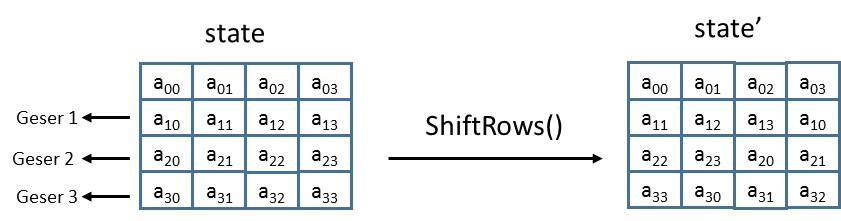
\includegraphics[width=0.85\textwidth]{../../images/python/page_059_img_01.jpeg}

\end{document}
